\documentclass[11pt]{article}
\usepackage[utf8]{inputenc}
\usepackage[spanish]{babel}
\decimalpoint
\usepackage{amsmath}
\usepackage{amsthm}
\usepackage{amssymb}
\usepackage{graphicx}
\usepackage[margin=0.8in]{geometry}
\usepackage{fancyhdr}
\usepackage[inline]{enumitem}
\usepackage{float}
\usepackage{cancel}
\usepackage{bigints}
\usepackage{listings}
\usepackage{xcolor}
\usepackage{listingsutf8}
\usepackage{algpseudocode}
\usepackage{algorithm}
\usepackage{apacite}
\usepackage{tcolorbox}
\usepackage{multicol}
\usepackage{tipa}
\usepackage{caption} 
\pagestyle{fancy}
\usepackage{hyperref}
\usepackage{amsmath}
\usepackage{mathtools}% http://ctan.org/pkg/mathtools
\hypersetup{
    colorlinks,
    citecolor=black,
    filecolor=black,
    linkcolor=black,
    urlcolor=black
}
\newcommand{\xvdash}[1]{%
	\vdash^{\mkern-10mu\scriptscriptstyle\rule[-.9ex]{0pt}{0pt}#1}%
}
\setlength{\headheight}{15pt} 
\lhead{Ecuaciones simbólicas de los ECA para la regla 22 y 54}
\rhead{\thepage}
\lfoot{ESCOM-IPN}
\renewcommand{\footrulewidth}{0.5pt}
\setlength{\parskip}{0.5em}
\newcommand{\ve}[1]{\overrightarrow{#1}}
\newcommand{\abs}[1]{\left\lvert #1 \right\lvert}
\newcommand{\blank}{\text{\textcrb}}
\date{\today}
\title{Ecuaciones simbólicas de los ECA para la regla 22 y 54}
\author{Sanchez Mendez Edmundo Josue}

\lstdefinestyle{customc}{
	belowcaptionskip=1\baselineskip,
	breaklines=true,
	frame=L,
	xleftmargin=\parindent,
	language=C++,
	showstringspaces=false,
	basicstyle=\ttfamily,
	keywordstyle=\bfseries\color{green!40!black},
	commentstyle=\itshape\color{purple!40!black},
	identifierstyle=\color{blue},
	numbers=left,
	stringstyle=\color{orange},
}

\lstset{escapechar=@,style=customc,tabsize=3,language=C++}

\bibliographystyle{apacite}
\begin{document}
		\begin{titlepage}
			\begin{center}
				
				% Upper part of the page. The '~' is needed because \\
				% only works if a paragraph has started.
				
				\noindent
				\begin{minipage}{0.5\textwidth}
					\begin{flushleft} \large
						
\includegraphics[width=0.5\textwidth]{resources/ipn.png}
					\end{flushleft}
				\end{minipage}%
				\begin{minipage}{0.55\textwidth}
					\begin{flushright} \large
						
\includegraphics[width=0.5\textwidth]{resources/escom.png}
					\end{flushright}
				\end{minipage}
				
				\textsc{\LARGE Instituto Politécnico Nacional}\\[0.5cm]
				
				\textsc{\Large Escuela Superior de Cómputo}\\[1cm]
				
				% Title
				
				{ \huge Ecuaciones simbólicas de los ECA para la regla 22 y 54  \\[1cm] }
				
				{ \Large Unidad de aprendizaje: Computing Selected Topics} \\[1cm]
				
				{ \Large Grupo: 3CM19 } \\[1cm]
				
				\noindent
				\begin{minipage}{0.5\textwidth}
					\begin{flushleft} \large
						\emph{Alumno:} \\
						Sanchez Mendez Edmundo Josue
					\end{flushleft}
				\end{minipage}%
				\begin{minipage}{0.5\textwidth}
					\begin{flushright} \large
						\emph{Profesor:} \\
						Juarez Martinez Genaro
					\end{flushright}
				\end{minipage}
				
				\vfill
				% Bottom of the page
				{\large {\today}}
			\end{center}
		\end{titlepage}
	
	\titlepage
	\tableofcontents
	\newpage
	
	\section{Introducción}
		En este documento se harán los cálculos correspondientes para hallar las ecuaciones simbólicas de un autómata celular elemental para la regla 22 y la regla 54 mediante el uso de la ecuación recursiva siguiente.
	\begin{equation}
		R_{ij}^{(k)}=R_{ij}^{(k-1)}+R_{ik}^{(k-1)}{(R_{kk}^{(k-1)})}^\ast R_{kj}^{(k-1)}
	\end{equation}

	\section{Ecuaciones simbólicas regla 22}
	Para poder encontrar una ecuación que describa a nuestro autómata necesitaremos el diagrama de 'de Bruijn' de nuestro ECA para la regla 22, el cual es el que se representa en la figura 1.
	\begin{figure}[H]
			\centering
			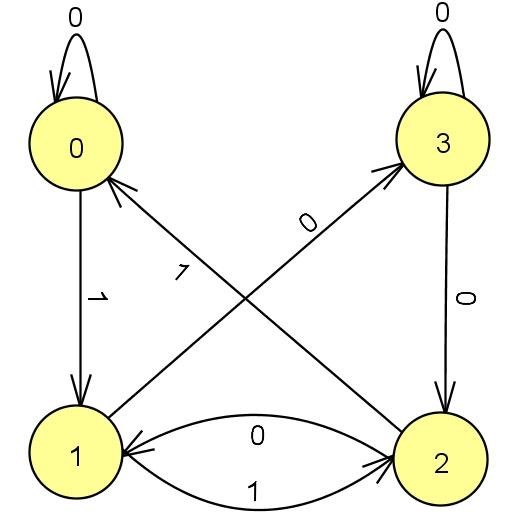
\includegraphics[scale=0.5]{resources/rule22f.jpg}
			\caption{Diagrama de 'de Bruijn' para ECA regla 22}\label{fig:picture}
	\end{figure}
		\subsection{Cálculos para k=0}
			\[R_{00}^{(0)}=\varepsilon+0; R_{01}^{(0)}=1; R_{02}^{(0)}=\emptyset;
			  R_{03}^{(0)}=\emptyset\]
			\[R_{10}^{(0)}=\emptyset; R_{11}^{(0)}=\varepsilon; R_{12}^{(0)}=1;
			  R_{13}^{(0)}=0\]
			\[R_{20}^{(0)}=1; R_{21}^{(0)}=0; R_{22}^{(0)}=\varepsilon;
			  R_{23}^{(0)}=\emptyset\]
			\[R_{30}^{(0)}=\emptyset; R_{31}^{(0)}=\emptyset; R_{32}^{(0)}=0;
			  R_{33}^{(0)}=\varepsilon+0\]
		\subsection{Cálculos para k=1}
			\[R_{00}^{(1)}=R_{00}^{0}+R_{01}^{0}{(R_{11}^{0})}^\ast R_{10}^{0}=(\varepsilon+0)+(1)(\varepsilon)^\ast(\emptyset)=\varepsilon+0\]
			\[R_{01}^{(1)}=R_{01}^{0}+R_{01}^{0}{(R_{11}^{0})}^\ast R_{11}^{0}=(1)+(1)(\varepsilon)^\ast(\varepsilon)=1\]
			\[R_{02}^{(1)}=R_{02}^{0}+R_{01}^{0}{(R_{11}^{0})}^\ast R_{12}^{0}=\emptyset+(1)(\varepsilon)^\ast(1)=11\]
			\[R_{03}^{(1)}=R_{03}^{0}+R_{01}^{0}{(R_{11}^{0})}^\ast R_{13}^{0}=\emptyset+(1)(\varepsilon)^\ast(0)=10\]
			\[R_{10}^{(1)}=R_{10}^{0}+R_{11}^{0}{(R_{11}^{0})}^\ast R_{10}^{0}=\emptyset+(\varepsilon)(\varepsilon)^\ast(\emptyset)=\emptyset\]
			\[R_{11}^{(1)}=R_{11}^{0}+R_{11}^{0}{(R_{11}^{0})}^\ast R_{11}^{0}=(\varepsilon)+(\varepsilon)(\varepsilon)^\ast(\varepsilon)=\varepsilon\]
			\[R_{12}^{(1)}=R_{12}^{0}+R_{11}^{0}{(R_{11}^{0})}^\ast R_{12}^{0}=(1)+(\varepsilon)(\varepsilon)^\ast(1)=1\]
			\[R_{13}^{(1)}=R_{13}^{0}+R_{11}^{0}{(R_{11}^{0})}^\ast R_{13}^{0}=(0)+(\varepsilon)(\varepsilon)^\ast(0)=0\]
			\[R_{20}^{(1)}=R_{20}^{0}+R_{21}^{0}{(R_{11}^{0})}^\ast R_{10}^{0}=1+(0)(\varepsilon)^\ast(\emptyset)=1\]
			\[R_{21}^{(1)}=R_{21}^{0}+R_{21}^{0}{(R_{11}^{0})}^\ast R_{11}^{0}=(0)+(0)(\varepsilon)^\ast(\varepsilon)=0\]
			\[R_{22}^{(1)}=R_{22}^{0}+R_{21}^{0}{(R_{11}^{0})}^\ast R_{12}^{0}=(\varepsilon)+(0)(\varepsilon)^\ast(1)=\varepsilon+01\]
			\[R_{23}^{(1)}=R_{23}^{0}+R_{21}^{0}{(R_{11}^{0})}^\ast R_{13}^{0}=\emptyset+(0)(\varepsilon)^\ast(0)=00\]
			\[R_{30}^{(1)}=R_{30}^{0}+R_{31}^{0}{(R_{11}^{0})}^\ast R_{10}^{0}=\emptyset+(\emptyset)(\varepsilon)^\ast(\emptyset)=\emptyset\]
			\[R_{31}^{(1)}=R_{31}^{0}+R_{31}^{0}{(R_{11}^{0})}^\ast R_{11}^{0}=\emptyset+(\emptyset)(\varepsilon)^\ast(\varepsilon)=\emptyset\]
			\[R_{32}^{(1)}=R_{32}^{0}+R_{31}^{0}{(R_{11}^{0})}^\ast R_{12}^{0}=0+(\emptyset)(\varepsilon)^\ast(1)=0\]
			\[R_{33}^{(1)}=R_{33}^{0}+R_{31}^{0}{(R_{11}^{0})}^\ast R_{13}^{0}=(\varepsilon+0)+(\emptyset)(\varepsilon)^\ast(0)=\varepsilon+0\]
		\subsection{Cálculos para k=2}
			\[R_{00}^{(2)}=R_{00}^{1}+R_{02}^{1}{(R_{22}^{1})}^\ast R_{20}^{1}=(\varepsilon+0)+(11)(\varepsilon+01)^\ast(1)=\varepsilon+0+11(01)^\ast1\]
			\[R_{01}^{(2)}=R_{01}^{1}+R_{02}^{1}{(R_{22}^{1})}^\ast R_{21}^{1}=(1)+(11)(\varepsilon+01)^\ast(0)=1+11(01)^\ast0\]
			\[R_{02}^{(2)}=R_{02}^{1}+R_{02}^{1}{(R_{22}^{1})}^\ast R_{22}^{1}=(11)+(11)(\varepsilon+01)^\ast(\varepsilon+01)=11(01)^\ast\]
			\[R_{03}^{(2)}=R_{03}^{1}+R_{02}^{1}{(R_{22}^{1})}^\ast R_{23}^{1}=(10)+(11)(\varepsilon+01)^\ast(00)=1(0+1(01)^\ast00)\]
			\[R_{10}^{(2)}=R_{10}^{1}+R_{12}^{1}{(R_{22}^{1})}^\ast R_{20}^{1}=\emptyset+(1)(\varepsilon+01)^\ast(1)=1(01)^\ast1\]
			\[R_{11}^{(2)}=R_{11}^{1}+R_{12}^{1}{(R_{22}^{1})}^\ast R_{21}^{1}=(\varepsilon)+(1)(\varepsilon+01)^\ast(0)=\varepsilon+1(01)^\ast0\]
			\[R_{12}^{(2)}=R_{12}^{1}+R_{12}^{1}{(R_{22}^{1})}^\ast R_{22}^{1}=(1)+(1)(\varepsilon+01)^\ast(\varepsilon+01)=1(01)^\ast\]
			\[R_{13}^{(2)}=R_{13}^{1}+R_{12}^{1}{(R_{22}^{1})}^\ast R_{23}^{1}=0+(1)(\varepsilon+01)^\ast(00)=0+1(01)^\ast00\]
			\[R_{20}^{(2)}=R_{20}^{1}+R_{22}^{1}{(R_{22}^{1})}^\ast R_{20}^{1}=1+(\varepsilon+01)(\varepsilon+01)^\ast(1)=(01)^\ast1\]
			\[R_{21}^{(2)}=R_{21}^{1}+R_{22}^{1}{(R_{22}^{1})}^\ast R_{21}^{1}=0+(\varepsilon+01)(\varepsilon+01)^\ast(0)=(01)^\ast0\]
			\[R_{22}^{(2)}=R_{22}^{1}+R_{22}^{1}{(R_{22}^{1})}^\ast R_{22}^{1}=(\varepsilon+01)+(\varepsilon+01)(\varepsilon+01)^\ast(\varepsilon+01)=(01)^\ast\]
			\[R_{23}^{(2)}=R_{23}^{1}+R_{22}^{1}{(R_{22}^{1})}^\ast R_{23}^{1}=00+(\varepsilon+01)(\varepsilon+01)^\ast(00)=(01)^\ast00\]
			\[R_{30}^{(2)}=R_{30}^{1}+R_{32}^{1}{(R_{22}^{1})}^\ast R_{20}^{1}=\emptyset+(0)(\varepsilon+01)^\ast(1)=0(01)^\ast1\]
			\[R_{31}^{(2)}=R_{31}^{1}+R_{32}^{1}{(R_{22}^{1})}^\ast R_{21}^{1}=\emptyset+(0)(\varepsilon+01)^\ast(0)=0(01)^\ast0\]
			\[R_{32}^{(2)}=R_{32}^{1}+R_{32}^{1}{(R_{22}^{1})}^\ast R_{22}^{1}=0+(0)(\varepsilon+01)^\ast(\varepsilon+01)=0(01)^\ast\]
			\[R_{33}^{(2)}=R_{33}^{1}+R_{32}^{1}{(R_{22}^{1})}^\ast R_{23}^{1}=(\varepsilon+0)+(0)(\varepsilon+01)^\ast(00)=\varepsilon+0+0(01)^\ast00\]
		\subsection{Cálculos para k=3}
			\begin{multline*}
			R_{00}^{(3)}=R_{00}^{2}+R_{03}^{2}{(R_{33}^{2})}^\ast R_{30}^{2}=(\varepsilon+0+11(01)^\ast1)+(1(0+1(01)^\ast00))(\varepsilon+0+0(01)^\ast00)^\ast(0(01)^\ast1)=\\\varepsilon+0+1(1+(0+1(01)^\ast00)(0+0(01)^\ast00)^\ast0)(01)^\ast1
			\end{multline*}
			\begin{multline*}
			R_{01}^{(3)}=R_{01}^{2}+R_{03}^{2}{(R_{33}^{2})}^\ast R_{31}^{2}=(1+11(01)^\ast0)+(1(0+1(01)^\ast00))(\varepsilon+0+0(01)^\ast00)^\ast(0(01)^\ast0)=\\1+1(1+(0+1(01)^\ast00)(0+0(01)^\ast00)^\ast0)(01)^\ast0
			\end{multline*}
			\begin{multline*}
			R_{02}^{(3)}=R_{02}^{2}+R_{03}^{2}{(R_{33}^{2})}^\ast R_{32}^{2}=(11(01)^\ast)+(1(0+1(01)^\ast00))(\varepsilon+0+0(01)^\ast00)^\ast(0(01)^\ast)=\\1(1+(0+1(01)^\ast00)(0+0(01)^\ast00)^\ast0)(01)^\ast
			\end{multline*}
			\begin{multline*}
			R_{03}^{(3)}=R_{03}^{2}+R_{03}^{2}{(R_{33}^{2})}^\ast R_{33}^{2}=(1(0+1(01)^\ast00))+(1(0+1(01)^\ast00))(\varepsilon+0+0(01)^\ast00)^\ast(\varepsilon+0+0(01)^\ast00)=\\1(0+1(01)^\ast00)(0+0(01)^\ast00)^\ast
			\end{multline*}
			\begin{multline*}
			R_{10}^{(3)}=R_{10}^{2}+R_{13}^{2}{(R_{33}^{2})}^\ast R_{30}^{2}=(1(01)^\ast1)+(0+1(01)^\ast00)(\varepsilon+0+0(01)^\ast00)^\ast(0(01)^\ast1)=\\(1+(0+1(01)^\ast00)(0+0(01)^\ast00)^\ast0)(01)^\ast1
			\end{multline*}
			\begin{multline*}
			R_{11}^{(3)}=R_{11}^{2}+R_{13}^{2}{(R_{33}^{2})}^\ast R_{31}^{2}=(\varepsilon+1(01)^\ast0)+(0+1(01)^\ast00)(\varepsilon+0+0(01)^\ast00)^\ast(0(01)^\ast0)=\\\varepsilon+(1+(0+1(01)^\ast00)(0+0(01)^\ast00)^\ast0)(01)^\ast0
			\end{multline*}
			\begin{multline*}
			R_{12}^{(3)}=R_{12}^{2}+R_{13}^{2}{(R_{33}^{2})}^\ast R_{32}^{2}=(1(01)^\ast)+(0+1(01)^\ast00)(\varepsilon+0+0(01)^\ast00)^\ast(0(01)^\ast)=\\(1+(0+1(01)^\ast00)(0+0(01)^\ast00)^\ast0)(01)^\ast
			\end{multline*}
			\begin{multline*}	
			R_{13}^{(3)}=R_{13}^{2}+R_{13}^{2}{(R_{33}^{2})}^\ast R_{33}^{2}=(0+1(01)^\ast00)+(0+1(01)^\ast00)(\varepsilon+0+0(01)^\ast00)^\ast(\varepsilon+0+0(01)^\ast00)=\\(0+1(01)^\ast00)(0+0(01)^\ast00)^\ast
			\end{multline*}
			\begin{multline*}	
			R_{20}^{(3)}=R_{20}^{2}+R_{23}^{2}{(R_{33}^{2})}^\ast R_{30}^{2}=((01)^\ast1)+((01)^\ast00)(\varepsilon+0+0(01)^\ast00)^\ast(0(01)^\ast1)=\\(01)^\ast(1+00(0+0(01)^\ast00)^\ast0(01)^\ast1)
			\end{multline*}
			\begin{multline*}
			R_{21}^{(3)}=R_{21}^{2}+R_{23}^{2}{(R_{33}^{2})}^\ast R_{31}^{2}=((01)^\ast0)+((01)^\ast00)(\varepsilon+0+0(01)^\ast00)^\ast(0(01)^\ast0)=\\(01)^\ast(0+00(0+0(01)^\ast00)^\ast0(01)^\ast0)
			\end{multline*}
			\begin{multline*}
			R_{22}^{(3)}=R_{22}^{2}+R_{23}^{2}{(R_{33}^{2})}^\ast R_{32}^{2}=((01)^\ast)+((01)^\ast00)(\varepsilon+0+0(01)^\ast00)^\ast(0(01)^\ast)=\\(01)^\ast+(01)^\ast00(0+0(01)^\ast00)^\ast0(01)^\ast
			\end{multline*}
			\begin{multline*}
			R_{23}^{(3)}=R_{23}^{2}+R_{23}^{2}{(R_{33}^{2})}^\ast R_{33}^{2}=((01)^\ast00)+((01)^\ast00)(\varepsilon+0+0(01)^\ast00)^\ast(\varepsilon+0+0(01)^\ast00)=(01)^\ast00(0+0(01)^\ast00)^\ast)
			\end{multline*}
			\begin{multline*}
			R_{30}^{(3)}=R_{30}^{2}+R_{33}^{2}{(R_{33}^{2})}^\ast R_{30}^{2}=(0(01)^\ast1)+(\varepsilon+0+0(01)^\ast00)(\varepsilon+0+0(01)^\ast00)^\ast(0(01)^\ast1)=(0+0(01)^\ast00)^\ast0(01)^\ast1
			\end{multline*}
			\begin{multline*}
			R_{31}^{(3)}=R_{31}^{2}+R_{33}^{2}{(R_{33}^{2})}^\ast R_{31}^{2}=(0(01)^\ast0)+(\varepsilon+0+0(01)^\ast00)(\varepsilon+0+0(01)^\ast00)^\ast(0(01)^\ast0)=(0+0(01)^\ast00)^\ast0(01)^\ast0
			\end{multline*}
			\begin{multline*}
			R_{32}^{(3)}=R_{32}^{2}+R_{33}^{2}{(R_{33}^{2})}^\ast R_{32}^{2}=(0(01)^\ast)+(\varepsilon+0+0(01)^\ast00)(\varepsilon+0+0(01)^\ast00)^\ast(0(01)^\ast)=(0+0(01)^\ast00)^\ast0(01)^\ast
			\end{multline*}
			\begin{multline*}
			R_{33}^{(3)}=R_{33}^{2}+R_{33}^{2}{(R_{33}^{2})}^\ast R_{33}^{2}=(\varepsilon+0+0(01)^\ast00)+(\varepsilon+0+0(01)^\ast00)(\varepsilon+0+0(01)^\ast00)^\ast(\varepsilon+0+0(01)^\ast00)=\\(0+0(01)^\ast00)^\ast
			\end{multline*}
	\section{Ecuaciones simbólicas regla 54}
		Para poder encontrar una ecuación que describa a nuestro autómata necesitaremos el diagrama de 			'de Bruijn' de nuestro ECA para la regla 54, el cual es el que se representa en la figura 2.			\begin{figure}[H]
			\centering
			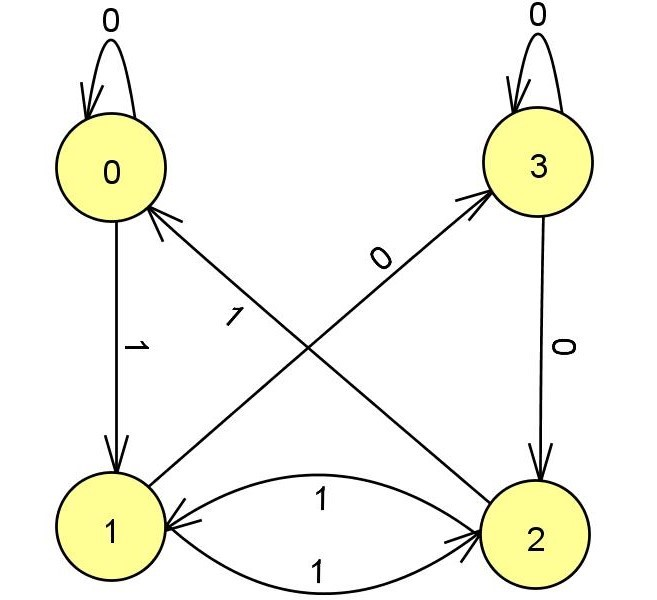
\includegraphics[scale=0.5]{resources/rule54f.jpg}
			\caption{Diagrama de 'de Bruijn' para uso de la ecuación 1 para ECA regla 54}\label{fig:picture}
		\end{figure}
		\subsection{Cálculos para k=0}
			\[R_{00}^{(0)}=\varepsilon+0; R_{01}^{(0)}=1; R_{02}^{(0)}=\emptyset;
			  R_{03}^{(0)}=\emptyset\]
			\[R_{10}^{(0)}=\emptyset; R_{11}^{(0)}=\varepsilon; R_{12}^{(0)}=1;
			  R_{13}^{(0)}=0\]
			\[R_{20}^{(0)}=1; R_{21}^{(0)}=1; R_{22}^{(0)}=\varepsilon;
			  R_{23}^{(0)}=\emptyset\]
			\[R_{30}^{(0)}=\emptyset; R_{31}^{(0)}=\emptyset; R_{32}^{(0)}=0;
			  R_{33}^{(0)}=\varepsilon+0\]
		\subsection{Cálculos para k=1}
			\[R_{00}^{(1)}=R_{00}^{0}+R_{01}^{0}{(R_{11}^{0})}^\ast R_{10}^{0}=(\varepsilon+0)+(1)(\varepsilon)^\ast(\emptyset)=\varepsilon+0\]
			\[R_{01}^{(1)}=R_{01}^{0}+R_{01}^{0}{(R_{11}^{0})}^\ast R_{11}^{0}=(1)+(1)(\varepsilon)^\ast(\varepsilon)=1\]
			\[R_{02}^{(1)}=R_{02}^{0}+R_{01}^{0}{(R_{11}^{0})}^\ast R_{12}^{0}=\emptyset+(1)(\varepsilon)^\ast(1)=11\]
			\[R_{03}^{(1)}=R_{03}^{0}+R_{01}^{0}{(R_{11}^{0})}^\ast R_{13}^{0}=\emptyset+(1)(\varepsilon)^\ast(0)=10\]
			\[R_{10}^{(1)}=R_{10}^{0}+R_{11}^{0}{(R_{11}^{0})}^\ast R_{10}^{0}=\emptyset+(\varepsilon)(\varepsilon)^\ast(\emptyset)=\emptyset\]
			\[R_{11}^{(1)}=R_{11}^{0}+R_{11}^{0}{(R_{11}^{0})}^\ast R_{11}^{0}=(\varepsilon)+(\varepsilon)(\varepsilon)^\ast(\varepsilon)=\varepsilon\]
			\[R_{12}^{(1)}=R_{12}^{0}+R_{11}^{0}{(R_{11}^{0})}^\ast R_{12}^{0}=(1)+(\varepsilon)(\varepsilon)^\ast(1)=1\]
			\[R_{13}^{(1)}=R_{13}^{0}+R_{11}^{0}{(R_{11}^{0})}^\ast R_{13}^{0}=(0)+(\varepsilon)(\varepsilon)^\ast(0)=0\]
			\[R_{20}^{(1)}=R_{20}^{0}+R_{21}^{0}{(R_{11}^{0})}^\ast R_{10}^{0}=1+(1)(\varepsilon)^\ast(\emptyset)=1\]
			\[R_{21}^{(1)}=R_{21}^{0}+R_{21}^{0}{(R_{11}^{0})}^\ast R_{11}^{0}=(1)+(1)(\varepsilon)^\ast(\varepsilon)=1\]
			\[R_{22}^{(1)}=R_{22}^{0}+R_{21}^{0}{(R_{11}^{0})}^\ast R_{12}^{0}=(\varepsilon)+(1)(\varepsilon)^\ast(1)=\varepsilon+11\]
			\[R_{23}^{(1)}=R_{23}^{0}+R_{21}^{0}{(R_{11}^{0})}^\ast R_{13}^{0}=\emptyset+(1)(\varepsilon)^\ast(0)=10\]
			\[R_{30}^{(1)}=R_{30}^{0}+R_{31}^{0}{(R_{11}^{0})}^\ast R_{10}^{0}=\emptyset+(\emptyset)(\varepsilon)^\ast(\emptyset)=\emptyset\]
			\[R_{31}^{(1)}=R_{31}^{0}+R_{31}^{0}{(R_{11}^{0})}^\ast R_{11}^{0}=\emptyset+(\emptyset)(\varepsilon)^\ast(\varepsilon)=\emptyset\]
			\[R_{32}^{(1)}=R_{32}^{0}+R_{31}^{0}{(R_{11}^{0})}^\ast R_{12}^{0}=0+(\emptyset)(\varepsilon)^\ast(1)=0\]
			\[R_{33}^{(1)}=R_{33}^{0}+R_{31}^{0}{(R_{11}^{0})}^\ast R_{13}^{0}=(\varepsilon+0)+(\emptyset)(\varepsilon)^\ast(0)=\varepsilon+0\]
		\subsection{Cálculos para k=2}
			\[R_{00}^{(2)}=R_{00}^{1}+R_{02}^{1}{(R_{22}^{1})}^\ast R_{20}^{1}=(\varepsilon+0)+(11)(\varepsilon+11)^\ast(1)=\varepsilon+0+11(11)^\ast1\]
			\[R_{01}^{(2)}=R_{01}^{1}+R_{02}^{1}{(R_{22}^{1})}^\ast R_{21}^{1}=(1)+(11)(\varepsilon+11)^\ast(1)=1+11(11)^\ast1\]
			\[R_{02}^{(2)}=R_{02}^{1}+R_{02}^{1}{(R_{22}^{1})}^\ast R_{22}^{1}=(11)+(11)(\varepsilon+11)^\ast(\varepsilon+11)=11(11)^\ast\]
			\[R_{03}^{(2)}=R_{03}^{1}+R_{02}^{1}{(R_{22}^{1})}^\ast R_{23}^{1}=(10)+(11)(\varepsilon+11)^\ast(10)=1(0+1(11)^\ast10)\]
			\[R_{10}^{(2)}=R_{10}^{1}+R_{12}^{1}{(R_{22}^{1})}^\ast R_{20}^{1}=\emptyset+(1)(\varepsilon+11)^\ast(1)=1(11)^\ast1\]
			\[R_{11}^{(2)}=R_{11}^{1}+R_{12}^{1}{(R_{22}^{1})}^\ast R_{21}^{1}=(\varepsilon)+(1)(\varepsilon+11)^\ast(1)=\varepsilon+1(11)^\ast1\]
			\[R_{12}^{(2)}=R_{12}^{1}+R_{12}^{1}{(R_{22}^{1})}^\ast R_{22}^{1}=(1)+(1)(\varepsilon+11)^\ast(\varepsilon+11)=1(11)^\ast\]
			\[R_{13}^{(2)}=R_{13}^{1}+R_{12}^{1}{(R_{22}^{1})}^\ast R_{23}^{1}=0+(1)(\varepsilon+11)^\ast(10)=0+1(11)^\ast10\]
			\[R_{20}^{(2)}=R_{20}^{1}+R_{22}^{1}{(R_{22}^{1})}^\ast R_{20}^{1}=1+(\varepsilon+11)(\varepsilon+11)^\ast(1)=(11)^\ast1\]
			\[R_{21}^{(2)}=R_{21}^{1}+R_{22}^{1}{(R_{22}^{1})}^\ast R_{21}^{1}=1+(\varepsilon+11)(\varepsilon+11)^\ast(1)=(11)^\ast1\]
			\[R_{22}^{(2)}=R_{22}^{1}+R_{22}^{1}{(R_{22}^{1})}^\ast R_{22}^{1}=(\varepsilon+11)+(\varepsilon+11)(\varepsilon+11)^\ast(\varepsilon+11)=(11)^\ast\]
			\[R_{23}^{(2)}=R_{23}^{1}+R_{22}^{1}{(R_{22}^{1})}^\ast R_{23}^{1}=10+(\varepsilon+11)(\varepsilon+11)^\ast(10)=(11)^\ast10\]
			\[R_{30}^{(2)}=R_{30}^{1}+R_{32}^{1}{(R_{22}^{1})}^\ast R_{20}^{1}=\emptyset+(0)(\varepsilon+11)^\ast(1)=0(11)^\ast1\]
			\[R_{31}^{(2)}=R_{31}^{1}+R_{32}^{1}{(R_{22}^{1})}^\ast R_{21}^{1}=\emptyset+(0)(\varepsilon+11)^\ast(1)=0(11)^\ast1\]
			\[R_{32}^{(2)}=R_{32}^{1}+R_{32}^{1}{(R_{22}^{1})}^\ast R_{22}^{1}=0+(0)(\varepsilon+11)^\ast(\varepsilon+11)=0(11)^\ast\]
			\[R_{33}^{(2)}=R_{33}^{1}+R_{32}^{1}{(R_{22}^{1})}^\ast R_{23}^{1}=(\varepsilon+0)+(0)(\varepsilon+11)^\ast(10)=\varepsilon+0+0(11)^\ast10\]
		\subsection{Cálculos para k=3}
			\begin{multline*}
			R_{00}^{(3)}=R_{00}^{2}+R_{03}^{2}{(R_{33}^{2})}^\ast R_{30}^{2}=(\varepsilon+0+11(11)^\ast1)+(1(0+1(11)^\ast10))(\varepsilon+0+0(11)^\ast10)^\ast(0(11)^\ast1)=\\\varepsilon+0+1(1+(0+1(11)^\ast10)(0+0(11)^\ast10)^\ast0)(11)^\ast1
			\end{multline*}
			\begin{multline*}
			R_{01}^{(3)}=R_{01}^{2}+R_{03}^{2}{(R_{33}^{2})}^\ast R_{31}^{2}=(1+11(11)^\ast1)+(1(0+1(11)^\ast10))(\varepsilon+0+0(11)^\ast10)^\ast(0(11)^\ast1)=\\1+1(1+(0+1(11)^\ast10)(0+0(11)^\ast10)^\ast0)(11)^\ast1
			\end{multline*}
			\begin{multline*}
			R_{02}^{(3)}=R_{02}^{2}+R_{03}^{2}{(R_{33}^{2})}^\ast R_{32}^{2}=(11(11)^\ast)+(1(0+1(11)^\ast10))(\varepsilon+0+0(11)^\ast10)^\ast(0(11)^\ast)=\\1(1+(0+1(11)^\ast10)(0+0(11)^\ast10)^\ast0)(11)^\ast
			\end{multline*}
			\begin{multline*}
			R_{03}^{(3)}=R_{03}^{2}+R_{03}^{2}{(R_{33}^{2})}^\ast R_{33}^{2}=(1(0+1(11)^\ast10))+(1(0+1(11)^\ast10))(\varepsilon+0+0(11)^\ast10)^\ast(\varepsilon+0+0(11)^\ast10)=\\1(0+1(11)^\ast10)(0+0(11)^\ast10)^\ast
			\end{multline*}
			\begin{multline*}
			R_{10}^{(3)}=R_{10}^{2}+R_{13}^{2}{(R_{33}^{2})}^\ast R_{30}^{2}=(1(11)^\ast1)+(0+1(11)^\ast10)(\varepsilon+0+0(11)^\ast10)^\ast(0(11)^\ast1)=\\(1+(0+1(11)^\ast10)(0+0(11)^\ast10)^\ast0)(11)^\ast1
			\end{multline*}
			\begin{multline*}
			R_{11}^{(3)}=R_{11}^{2}+R_{13}^{2}{(R_{33}^{2})}^\ast R_{31}^{2}=(\varepsilon+1(11)^\ast1)+(0+1(11)^\ast10)(\varepsilon+0+0(11)^\ast10)^\ast(0(11)^\ast1)=\\\varepsilon+(1+(0+1(11)^\ast10)(0+0(11)^\ast10)^\ast0)(11)^\ast1
			\end{multline*}
			\begin{multline*}
			R_{12}^{(3)}=R_{12}^{2}+R_{13}^{2}{(R_{33}^{2})}^\ast R_{32}^{2}=(1(11)^\ast)+(0+1(11)^\ast10)(\varepsilon+0+0(11)^\ast10)^\ast(0(11)^\ast)=\\(1+(0+1(11)^\ast10)(0+0(11)^\ast10)^\ast0)(11)^\ast
			\end{multline*}
			\begin{multline*}	
			R_{13}^{(3)}=R_{13}^{2}+R_{13}^{2}{(R_{33}^{2})}^\ast R_{33}^{2}=(0+1(11)^\ast10)+(0+1(11)^\ast10)(\varepsilon+0+0(11)^\ast10)^\ast(\varepsilon+0+0(11)^\ast10)=\\(0+1(11)^\ast10)(0+0(11)^\ast10)^\ast
			\end{multline*}
			\begin{multline*}	
			R_{20}^{(3)}=R_{20}^{2}+R_{23}^{2}{(R_{33}^{2})}^\ast R_{30}^{2}=((11)^\ast1)+((11)^\ast10)(\varepsilon+0+0(11)^\ast10)^\ast(0(11)^\ast1)=\\(11)^\ast(1+10(0+0(11)^\ast10)^\ast0(11)^\ast1)
			\end{multline*}
			\begin{multline*}
			R_{21}^{(3)}=R_{21}^{2}+R_{23}^{2}{(R_{33}^{2})}^\ast R_{31}^{2}=((11)^\ast1)+((11)^\ast10)(\varepsilon+0+0(11)^\ast10)^\ast(0(11)^\ast1)=\\(11)^\ast(1+10(0+0(11)^\ast10)^\ast0(11)^\ast1)
			\end{multline*}
			\begin{multline*}
			R_{22}^{(3)}=R_{22}^{2}+R_{23}^{2}{(R_{33}^{2})}^\ast R_{32}^{2}=((11)^\ast)+((11)^\ast10)(\varepsilon+0+0(11)^\ast10)^\ast(0(11)^\ast)=\\(11)^\ast+(11)^\ast10(0+0(11)^\ast10)^\ast0(11)^\ast
			\end{multline*}
			\begin{multline*}
			R_{23}^{(3)}=R_{23}^{2}+R_{23}^{2}{(R_{33}^{2})}^\ast R_{33}^{2}=((11)^\ast10)+((11)^\ast10)(\varepsilon+0+0(11)^\ast10)^\ast(\varepsilon+0+0(11)^\ast10)=(11)^\ast10(0+0(11)^\ast10)^\ast)
			\end{multline*}
			\begin{multline*}
			R_{30}^{(3)}=R_{30}^{2}+R_{33}^{2}{(R_{33}^{2})}^\ast R_{30}^{2}=(0(11)^\ast1)+(\varepsilon+0+0(11)^\ast10)(\varepsilon+0+0(11)^\ast10)^\ast(0(11)^\ast1)=(0+0(11)^\ast10)^\ast0(11)^\ast1
			\end{multline*}
			\begin{multline*}
			R_{31}^{(3)}=R_{31}^{2}+R_{33}^{2}{(R_{33}^{2})}^\ast R_{31}^{2}=(0(11)^\ast1)+(\varepsilon+0+0(11)^\ast10)(\varepsilon+0+0(11)^\ast10)^\ast(0(11)^\ast1)=(0+0(11)^\ast10)^\ast0(11)^\ast1
			\end{multline*}
			\begin{multline*}
			R_{32}^{(3)}=R_{32}^{2}+R_{33}^{2}{(R_{33}^{2})}^\ast R_{32}^{2}=(0(11)^\ast)+(\varepsilon+0+0(11)^\ast10)(\varepsilon+0+0(11)^\ast10)^\ast(0(11)^\ast)=(0+0(11)^\ast10)^\ast0(11)^\ast
			\end{multline*}
			\begin{multline*}
			R_{33}^{(3)}=R_{33}^{2}+R_{33}^{2}{(R_{33}^{2})}^\ast R_{33}^{2}=(\varepsilon+0+0(11)^\ast10)+(\varepsilon+0+0(11)^\ast10)(\varepsilon+0+0(11)^\ast10)^\ast(\varepsilon+0+0(11)^\ast10)=\\(0+0(11)^\ast10)^\ast
			\end{multline*}
	\section{Conclusiones}
	Como conclusión para este reporte se escriben las ecuaciones que describen a los autómatas celulares elementales para la regla 22 y 54.\par
		Ecuación para la regla 22:\[(0+1(01)^\ast00)(0+0(01)^\ast00)^\ast\]\par
	Ecuación para la regla 54: \[(0+1(11)^\ast10)(0+0(11)^\ast10)^\ast\]
	\begin{thebibliography}{1}
 \bibitem[label1]{cite_key1} Martínez, G., Adamatzky, A., Hoffmann, R., Désérable, D. and Zelinka, I., 2019. On Patterns and Dynamics of Rule 22 Cellular Automaton. [ebook] Available at: https://content.wolfram.com/uploads/sites/13/2019/06/28-2-1.pdf [Accessed 5 May 2021]..	
 \bibitem[label2]{cite_key2} Martínez, G., Andrew, A. and McIntosh, H., 2018. Complete Characterization of Structure of Rule 54. [ebook] Available at: https://content.wolfram.com/uploads/sites/13/2018/12/23-3-4.pdf [Accessed 5 May 2021]..
\end{thebibliography}

\end{document}
